\section{Descrizione progetto}

\begin{figure}[h!]
      \centering
      \subfloat[\texttt{Homepage} della versione \textit{tablet} di {\movi}]{
          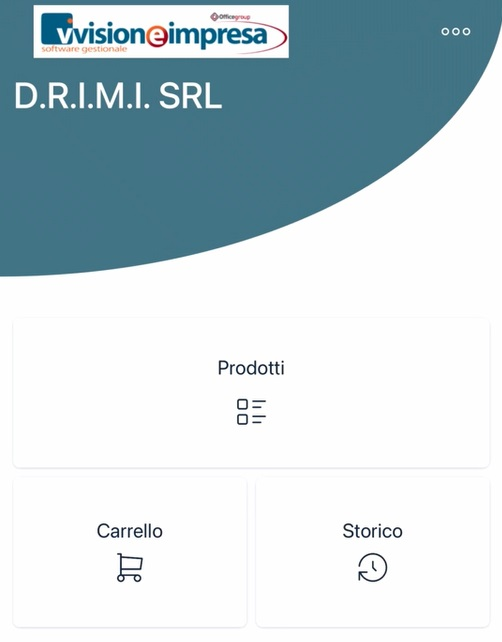
\includegraphics[width=0.45\textwidth]{img/MVOR_originale.jpg}
          \label{fig:MVOR originale}
      }
      \hfill
      \subfloat[Pagina \texttt{Prodotti} della versione \textit{smartphone} di {\movi}]{
          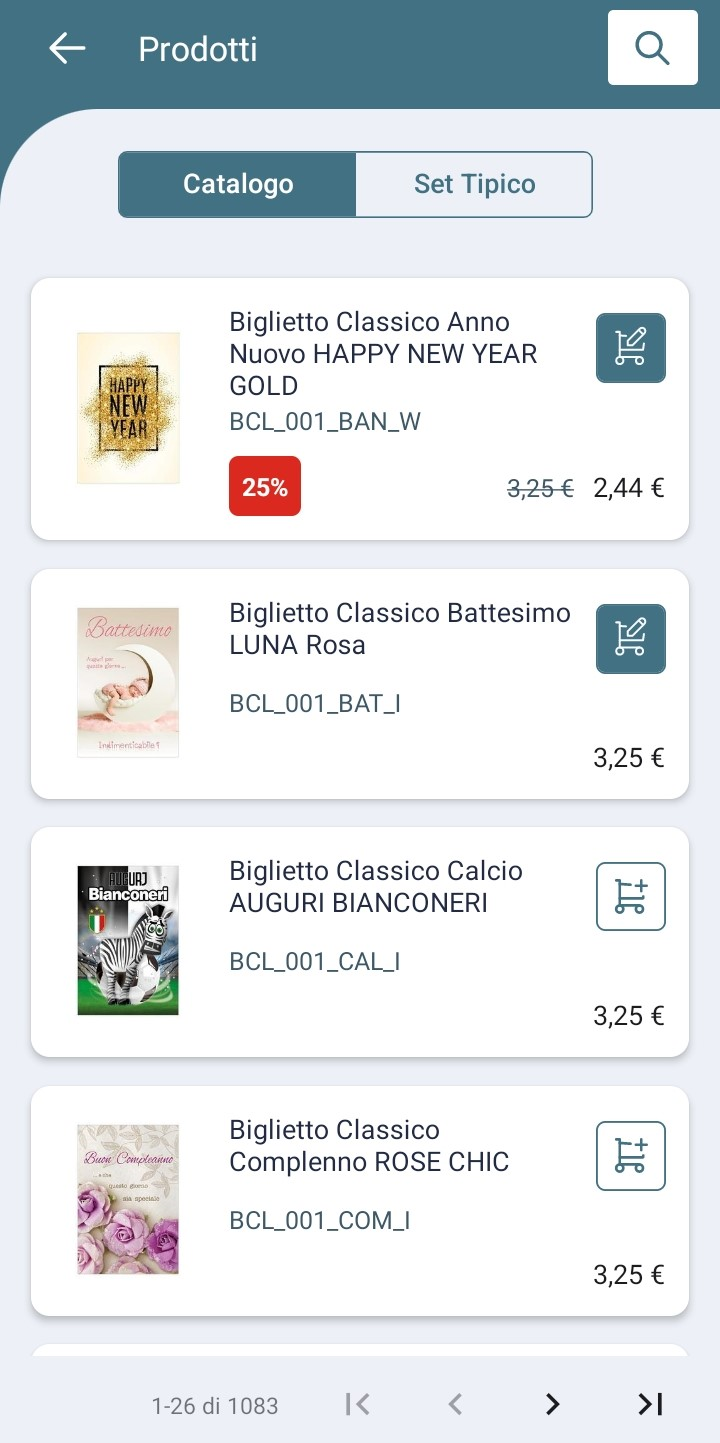
\includegraphics[width=0.3\textwidth]{img/MVOR_prodotti.jpg}
          \label{fig:MVOR prodotti}
      }
      \caption{Alcune \textit{view} di {\movi}}
      \label{fig:MVOR schermate}
\end{figure}

{\movi} è un'applicazione fornita dalle aziende ai loro clienti per gestire gli ordini ed effettuare il \textit{restock} della merce. 
L'\textit{app} permette inoltre di: visualizzare lo 
storico degli ordini precedenti, accedere a un \textit{set} tipico (ovvero un ordine predefinito con i prodotti solitamente 
acquistati), visualizzare il carrello per il riepilogo dell'ordine e uno storico dei 
documenti generati dopo la conferma dell'ordine.\\
La sua 
\texttt{Homepage} è visibile in figura \ref{fig:MVOR originale}, mentre il catalogo prodotti è mostrato in figura 
\ref{fig:MVOR prodotti}.\\
Il progetto assegnatomi da {\company} richiede di sviluppare un modulo per {\movi} chiamato "Modulo Agenti", ovvero 
l'insieme di interfacce, funzioni, \gls{api}, ecc. che permettono l'autenticazione di un nuovo tipo di utente, gli agenti aziendali, 
i quali, selezionando da una lista uno dei clienti a loro assegnati, possono operare nell'\textit{app} come il cliente selezionato.\\
La necessità di implementare questo modulo nasce da alcuni bisogni segnalati dai suoi clienti a {\company} e che 
mi sono stati descritti durante il primo incontro in azienda con il \textit{tutor} aziendale. I principali motivi sono:
\begin{itemize}
    \item \textbf{MoviSELL, l'\textit{app} pensata per gli agenti aziendali, è disponibile solo per \textit{tablet} iOS}. Questo può costituire un problema 
          per alcune aziende che, per dotare i propri agenti dell'\textit{app}, sono obbligate ad acquistare questi \textit{tablet} per i propri agenti. 
          Per aziende con agenti plurimandatari, cioè che rappresentano più aziende contemporaneamente, questo requisito si 
          rivela essere particolarmente oneroso da soddisfare, dato che si richiede di fornire i \textit{tablet} non ai propri dipendenti, 
          ma a professionisti esterni;
    \item \textbf{Non tutti gli agenti si trovano a loro agio ad usare il \textit{tablet}}, trovandolo ingombrante e scomodo, soprattutto per chi 
          lavora molto in mobilità. Pertanto, avere un'alternativa per smartphone risulta preferibile.
    \item MoviSELL è un'\textit{app} ricca di funzionalità, ma può risultare di difficile utilizzo per chi non ha dimestichezza con gli 
          strumenti digitali. \textbf{{\movi} risulta molto più semplice e intuitiva, rimuovendo la barriera tecnologica per alcuni 
          agenti} e permettendo loro di svolgere il loro lavoro;
    \item Alcuni clienti preferiscono contattare direttamente gli agenti per effettuare i loro ordini, invece di usare {\movi}. 
          \textbf{Il modulo agenti semplifica l'operazione di creazione dell'ordine per gli agenti}, evitando loro di dover appuntare 
          la merce da ordinare e poi effettuare l'ordine dal \textit{computer} una volta rientrati in ufficio.
\end{itemize}